\subsubsection{Software testing and devops practices used (D3)}
\label{testing_practices}

Testing is an important process in improving the quality of the software product. The purpose of this process is to find errors, which might occur during specification, design, and coding phases. We report the following results next:

\begin{itemize}
\item Software Testing Practices (Q 14)
\item Level of Automated Testing (Q 15)
\item Tools Used in Testing and QA (Q 16)
\item Continuous Deployment tools (Q 17)
\item Version Control (Q 18)
\end{itemize}


\paragraph{Software Testing Practices}
According to Figure \ref{fig:testing}, several testing practices are used during software development. The results show that most of the organizations have carried out unit testing (53\%), functional testing (49\%), user acceptance testing (39\%), GUI testing (31\%), etc. Unit testing also ranked first in the 2019 survey of JetBrains, where it was voted by 71\% participants across the globe \cite{JetBrains2019}. We observed in our survey that in some cases managers have reported performing GUI testing and performance testing, which is unlikely in their role/designation. However, the observation is not statistically significant ($p=0.12$). It may be deduced that in absence of enough specialized resource managers have to take additional responsibility. To identify the relation between testing practices and experience, we plotted them together in Figure \ref{fig:testing type and experience}. We have observed that junior developers mostly perform unit, integration, and functional testing, whereas senior developers mostly perform API testing. We conducted the Mann Whitney U test to assess the conjecture, and it is found statistically significant ($p<0.01$).

\begin{figure}[h]
\centering
  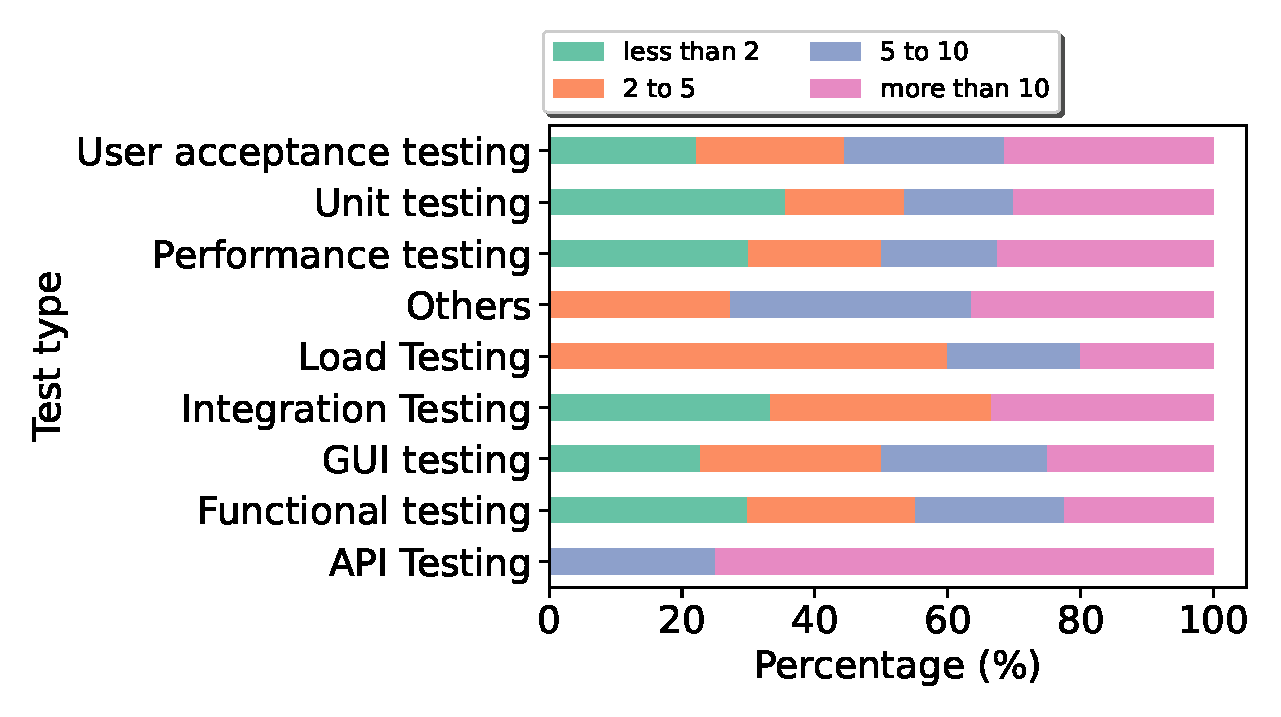
\includegraphics[scale=0.6]{Figures/Testing_Type_and_Experience}
  \caption{Testing practices ans professional experience}
  \label{fig:testing type and experience}
\end{figure}

\begin{figure}[h]
\centering
  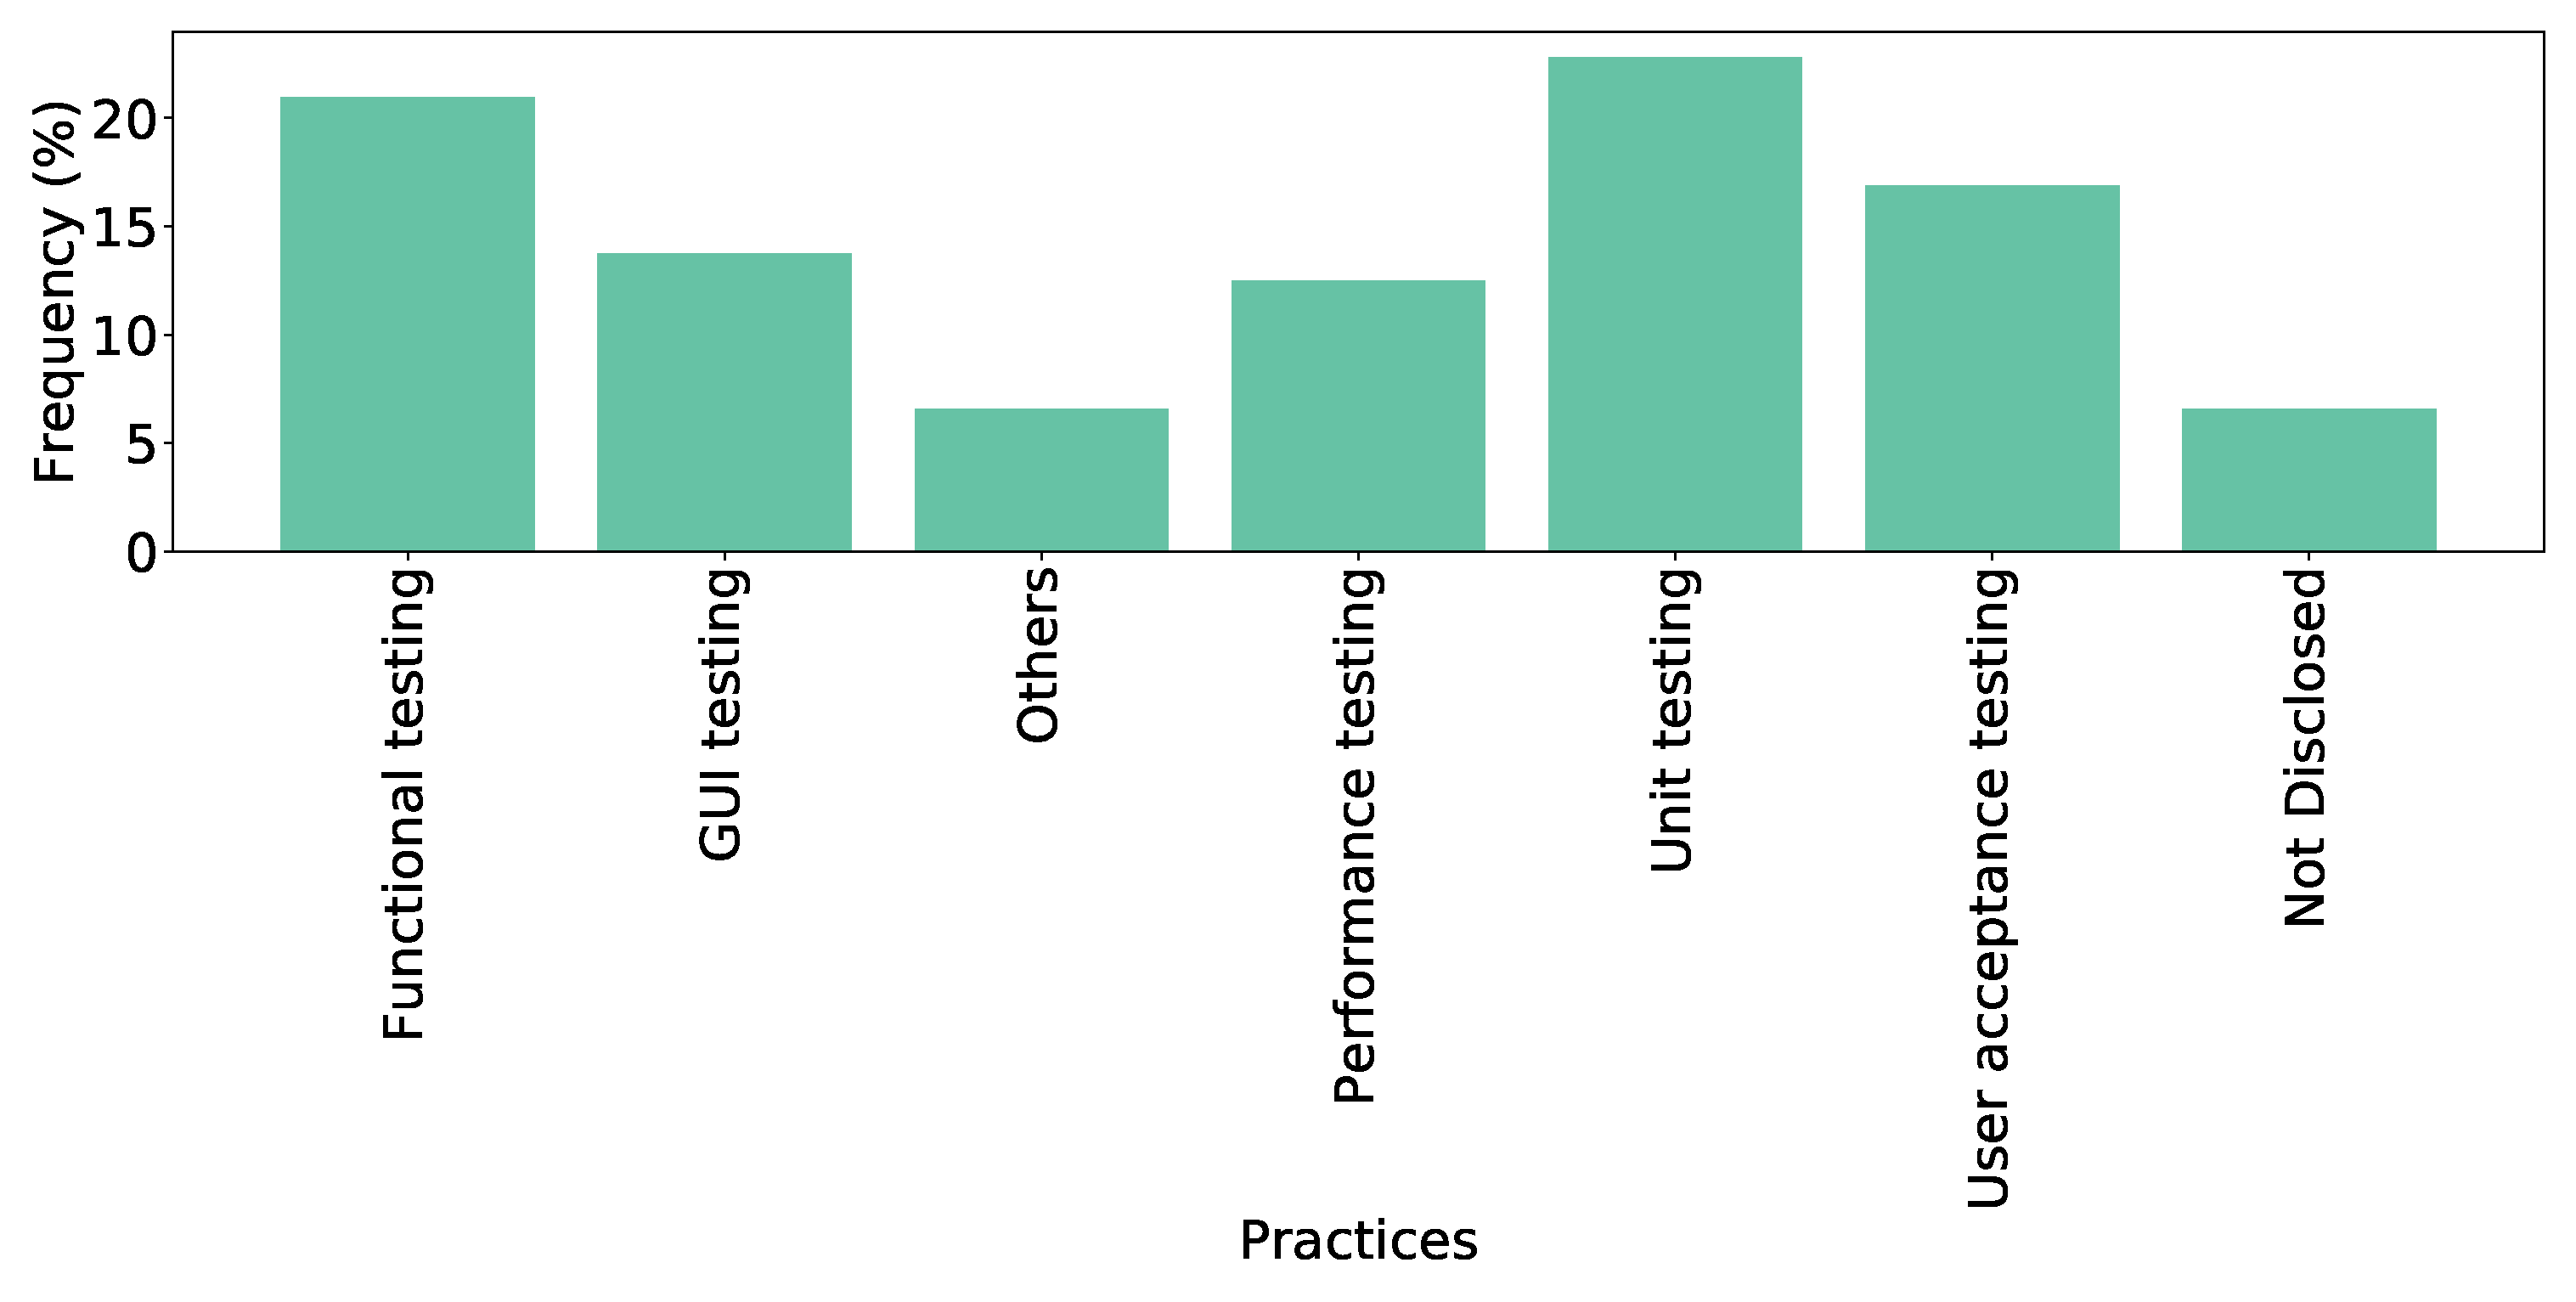
\includegraphics[scale=0.2]{Figures/Respondents_testing_practices}
  \caption{Testing Practices}
  \label{fig:testing}
\end{figure}

\paragraph{Level of Automated Testing}
We have asked the survey participants about the level of automated testing performed in their respective companies. The responses were gathered using the Likert scale. It was found that different respondents have very different experiences in this context, i.e., some companies heavily practice automated testing, while others favor manual testing.  Results are shown in Figure \ref{fig:autoTest}, which indicates that about 70\% of our respondents (others than who voted for level 5) do not use automated testing regularly. The level of automated testing might be related to the programming language/framework. The testing suite provided by framework/language might encourage developers to implement automated testing. The level of automated testing vs. language and framework is plotted in Figures \ref{fig:language and autotest} and \ref{fig:framework and autotest}, respectively. It seems from Figure \ref{fig:language and autotest} that the highest level of automated testing is mostly practiced in Java, JavaScript, Objective-C, and PHP language. We conducted the Mann Whitney U test to assess our conjecture and it is found statistically significant ($p=0.01$). From Figure \ref{fig:framework and autotest}, we found that the highest level of automated testing is mostly performed in Android, Express, Node.js, Struts, and Java EE framework, and the observation is statistically significant ($p=0.006$). Also, the highest level of automated testing is mainly used by developers (mostly use unit testing), and managers practice the lowest level of automated testing. The reason why managers use the lowest level of automated testing may be related to the type of testing they perform. We observed that managers mainly engaged in assessing the acceptability of the product from the end-user point of view. We guess that experience might be one of the factors that influence automated testing. Our conjecture was that senior developers might tend to use more automated tests than junior developers. We plotted experience and automated test levels in Figure \ref{fig:experience and autotest}. However, we found the opposite scenario, i.e., junior developers tend to use more automated testing than senior developers. However, the observation is not statistically significant ($p=0.08$). One of the reasons behind this observation may be that the senior developers perform certain testings (e.g., GUI testing), which are hard to automate.

\begin{figure}[h]
\centering
  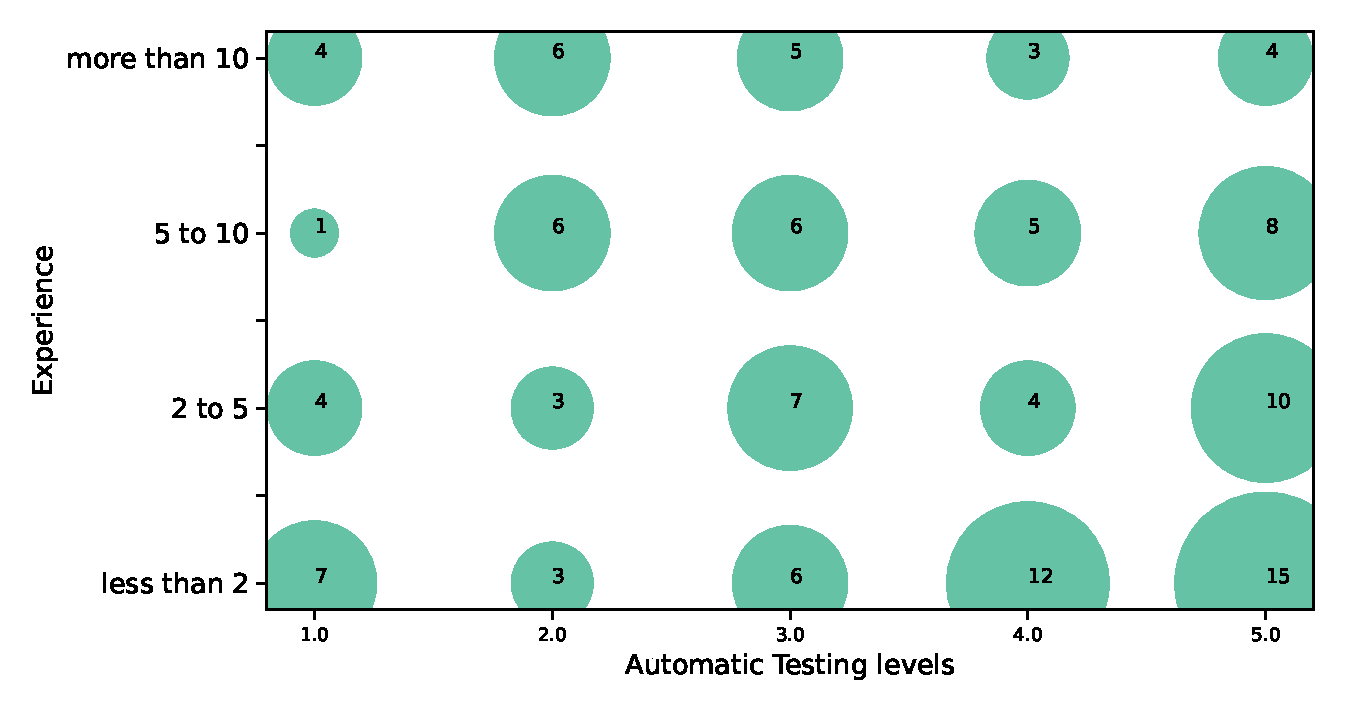
\includegraphics[scale=0.45]{Figures/Auto_Test_and_Experience}
  \caption{Experience and automated testing level}
  \label{fig:experience and autotest}
\end{figure}
\begin{figure}[h]
\centering
  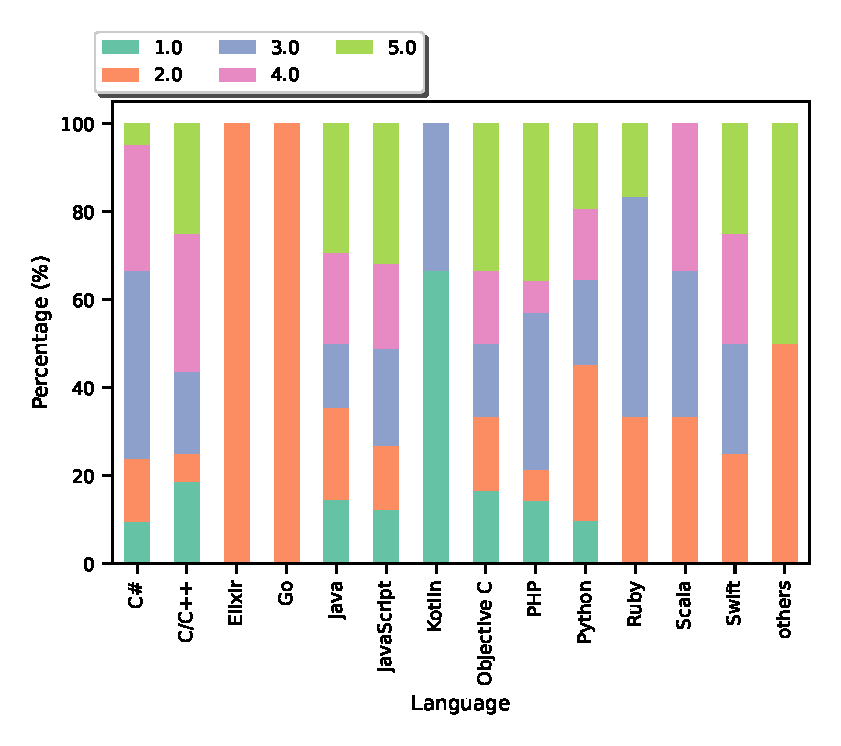
\includegraphics[scale=0.65]{Figures/Language_and_Test_Level}
  \caption{Programming language and automated testing level}
  \label{fig:language and autotest}
\end{figure}
\begin{figure}[h]
\centering
  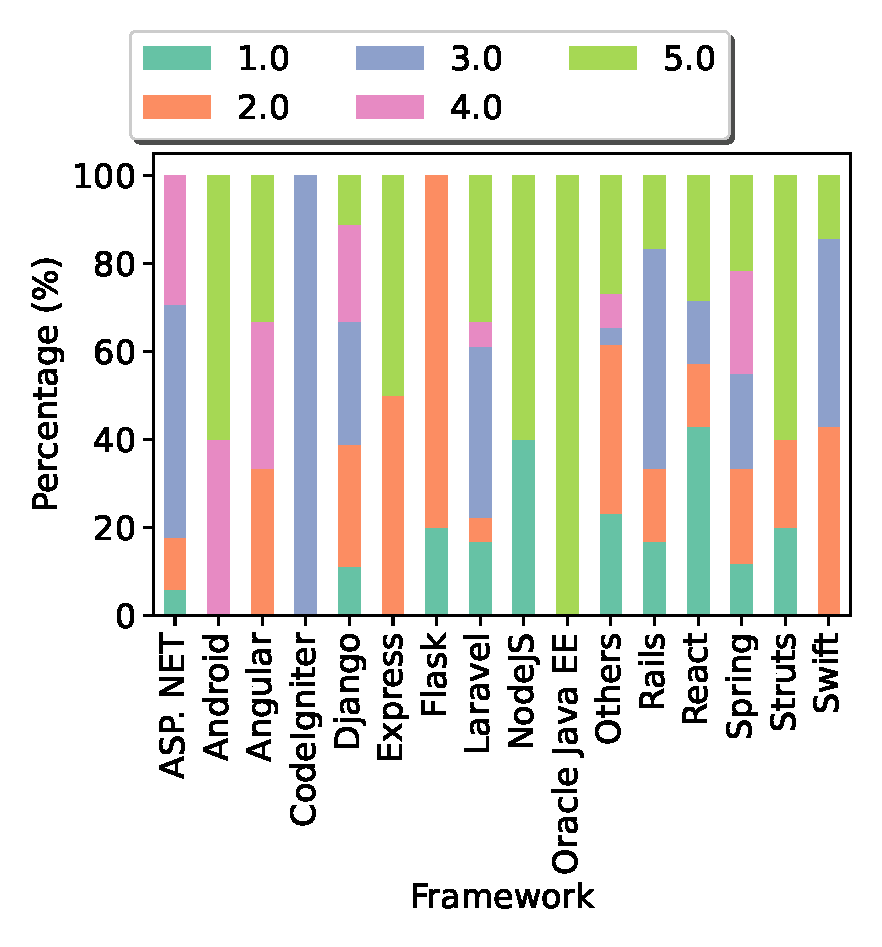
\includegraphics[scale=0.65]{Figures/Framework_and_Test_Level}
  \caption{Framework and automated testing level}
  \label{fig:framework and autotest}
\end{figure}

\begin{figure}[h]
\centering
  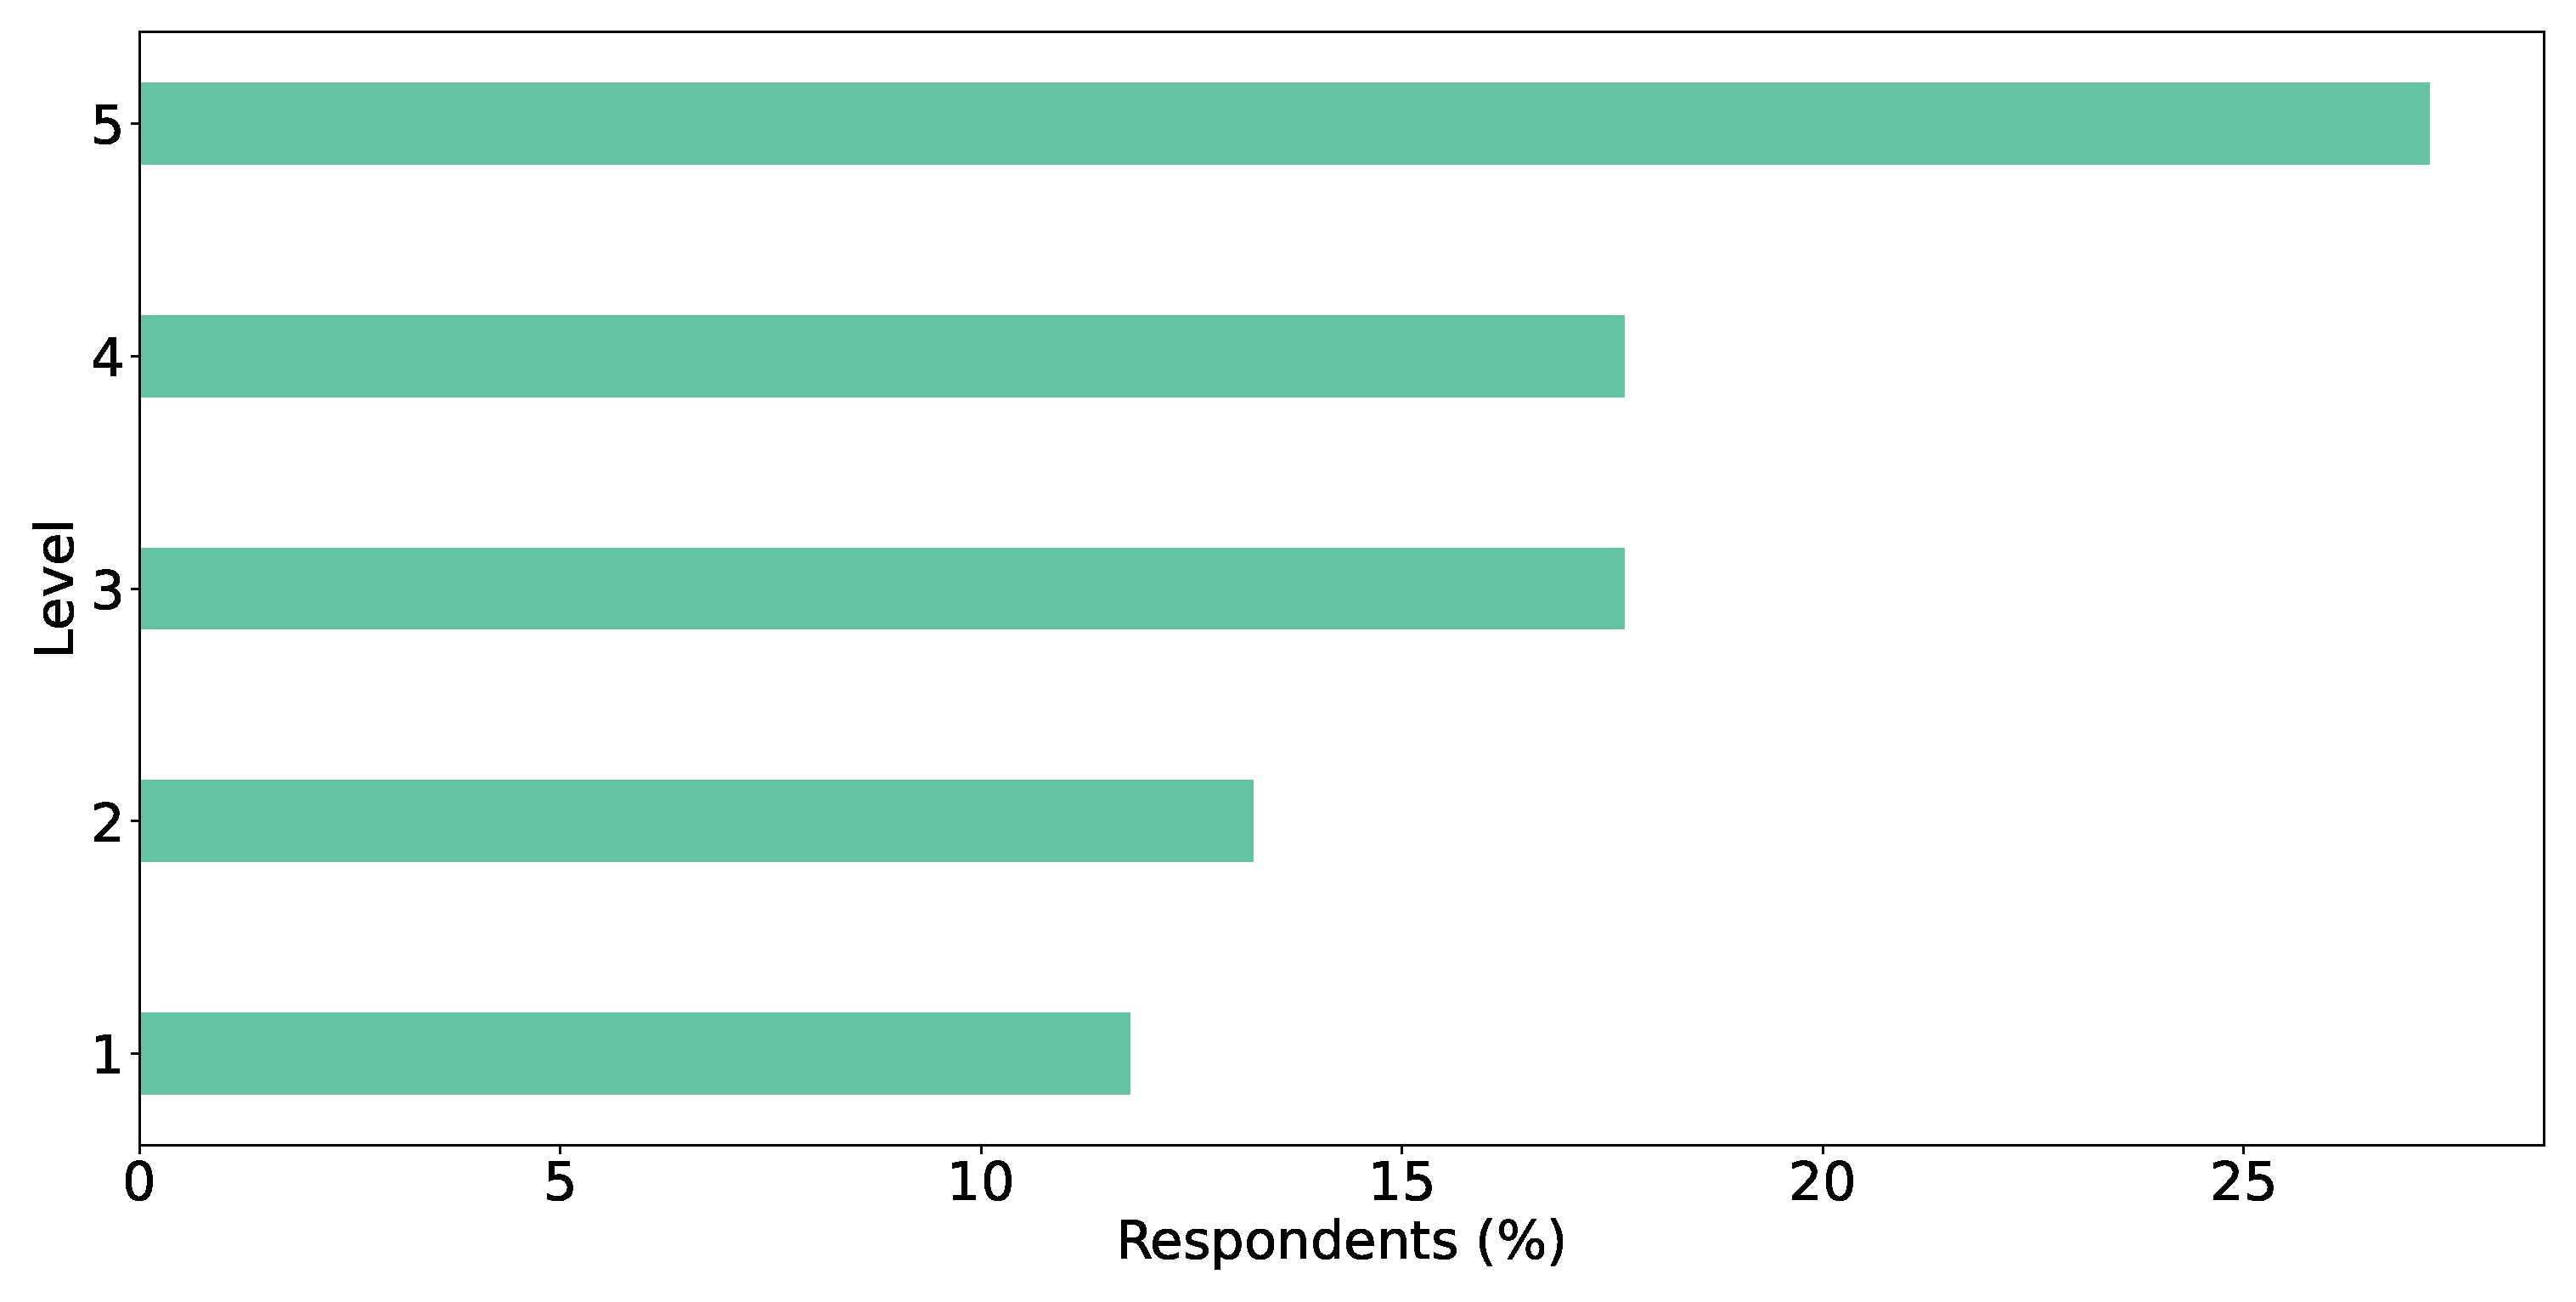
\includegraphics[scale=0.15]{Figures/Respondents_autotest_level}
  \caption{Automated Testing Level}
  \label{fig:autoTest}
\end{figure}

\boxtext{There is a tendency among most Bangladeshi developers not to use automated testing regularly.}
\anindya{Can it be the case that automated testing is done by SQA team, not regular developers?}


\paragraph{Tools Used in Testing and QA}
The survey participants were asked about the tools used in testing and quality assurance. According to \ref{fig:testingTools}, we see that most of the respondents have used XUnit( eg, JUnit, NUnit) (30\%), selenium (27\%), Jenkins (20\%), others (9\%). These results show that there exists a great demand for testing tools in the software industry of Bangladesh. However, around 38\% of our respondents were not interested in replying to this question that is not surprising because the majority of the respondents (93\% approx.) were working on roles other than SQA engineer as per Table \ref{tab:role}, and they are not supposed to be involved in any testing themselves. \anindya{This may be because many developers are not involved in any sort of testing themselves and our respondents are dominated by developers.} \khalid{added}

\begin{figure}[h]
\centering
  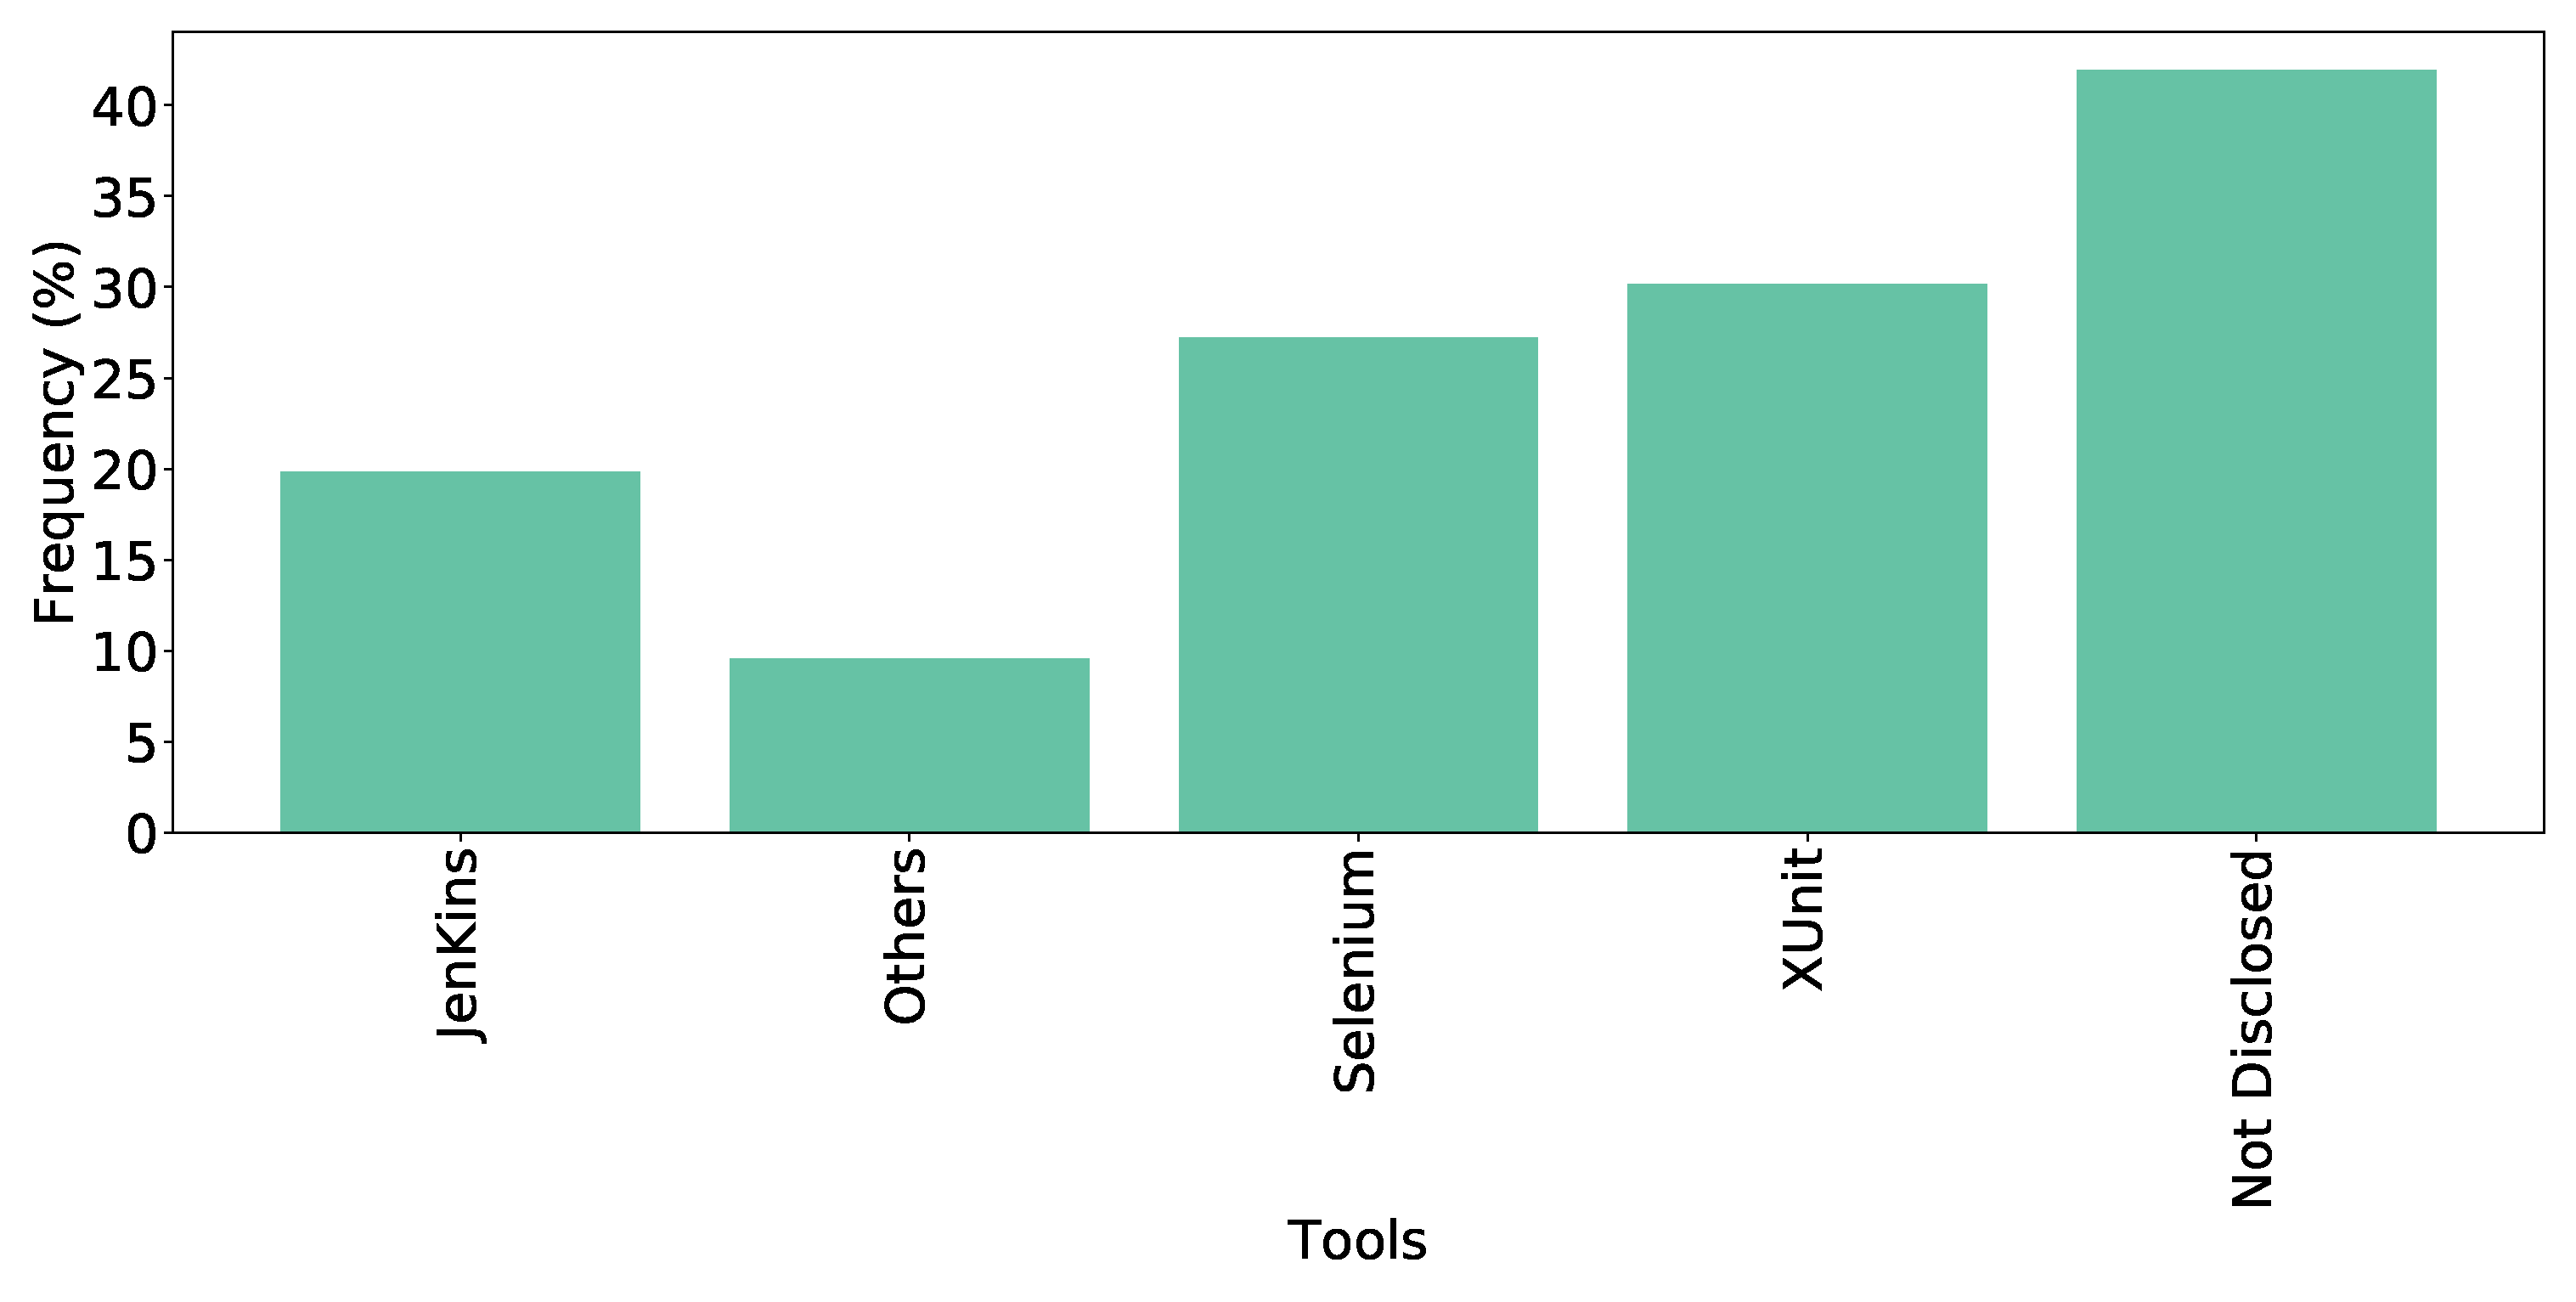
\includegraphics[scale=0.18]{Figures/Respondents_testing_tools}
  \caption{Testing \& QA Tools}
  \label{fig:testingTools}
\end{figure}

\boxtext{There has a large demand of software testing tools in Bangladesh.}


\paragraph{Deployment Tools}
According to \ref{fig:deployTools}, we see that the majority of the respondents deploy their implemented codes using AWS code-deploy (12\%) and Jenkins (12\%). The other deployment tools are Bamboo (5\%), TeamCity (4\%), Octopus (2\%), etc. Respondents voted none (4\%) as they didn't use any deployment tools and 53\% of the respondents were not interested in this topic. Anyhow, the percentage of uninterested respondents does not seem unexpected. From Table \ref{tab:role} and \ref{tab:experience}, we can observe that a significant portion of our respondents is developers, and more than half of our respondents are experienced for less than five years respectively. As deployment is related to DevOps, it is quite likely that developers have not enough knowledge or have less interest in deployment. \anindya{Again, this is mostly a dev op related issue and the developers are not likely to respond in this regard.} \khalid{added} The outcome indicates that the usage rate of deployment tools in Bangladesh for continuous integration and continuous deployment is yet to be widespread. We also guessed that the practice of using deployment tools might be done only by senior practitioners. However, the hypothesis is not statistically significant ($p=0.37$).
\rifat{We are saying implicitly that the survey is for developers, not for QA and DevOps engineers. Is it OK?}


\begin{figure}[h]
\centering
  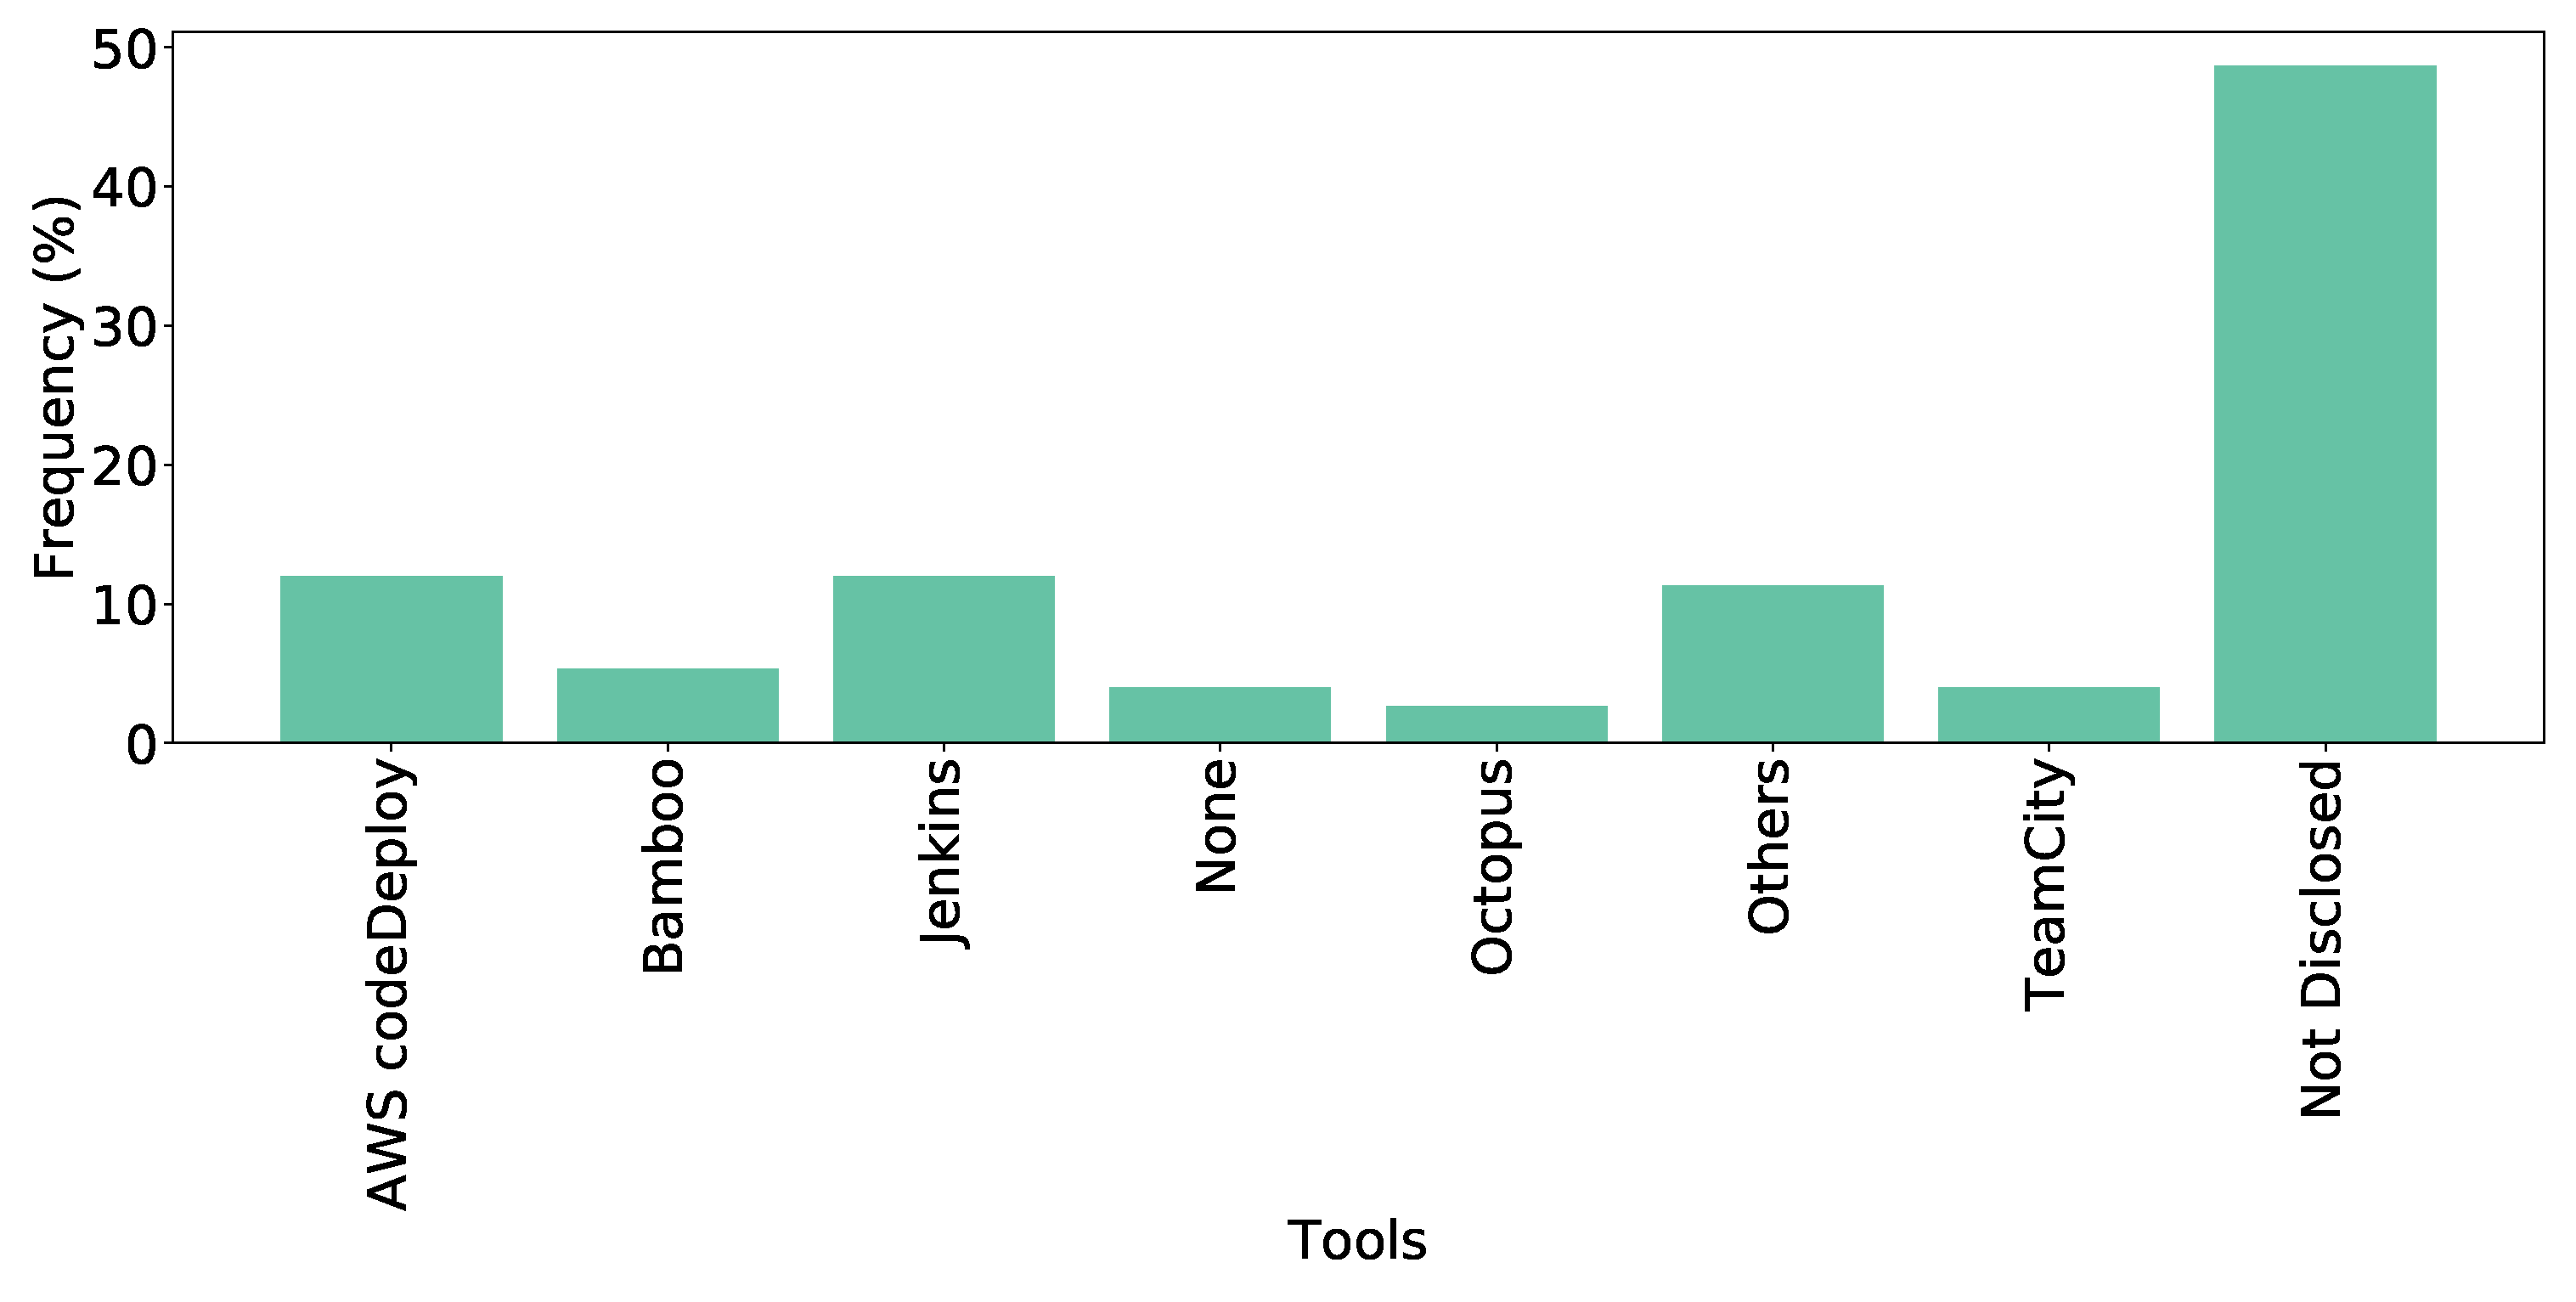
\includegraphics[scale=0.18]{Figures/Respondents_deployment_tools}
  \caption{Deployment Tools}
  \label{fig:deployTools}
\end{figure}


\paragraph{Version Control}
% \hfill\\
Git (78\%) and Bitbucket (29\%) are mostly-used version control systems in the software industry as shown in Figure \ref{fig:versionControl}. Besides these, Subversion (SVN) (5\%) and others (4\%) are used.  Respondents were allowed to select more than one option. The 2018 Stack overflow survey\cite{StackoverflowSurvey2018} reports that the most popular version control system is Git (87.2\% developer uses Git) and the second most popular is SVN (16.1\% developer uses SVN). However, in our survey, we found a slightly different result, the most popular version control system is Git and the second most popular is Bitbucket. This might be related to the declining popularity of SVN over the years. From the Stack overflow survey over the range 2017-2018, it is clear that SVN is losing popularity to Git. Nowadays, SVN is mainly used for versioning legacy projects. As the SE industry of Bangladesh is relatively young, this discrepancy observed is not surprising.
% \anindya{It looks nice that you compared with external relevant source like SO. Is it possible to do it for other RQs? Also, you may mention such deviations from other trends in Introduction.} \khalid{added in `methodologies', `tech platform', `test practices'} \partha{added in `os', `languages', `framework'}
\begin{figure}[h]
\centering
  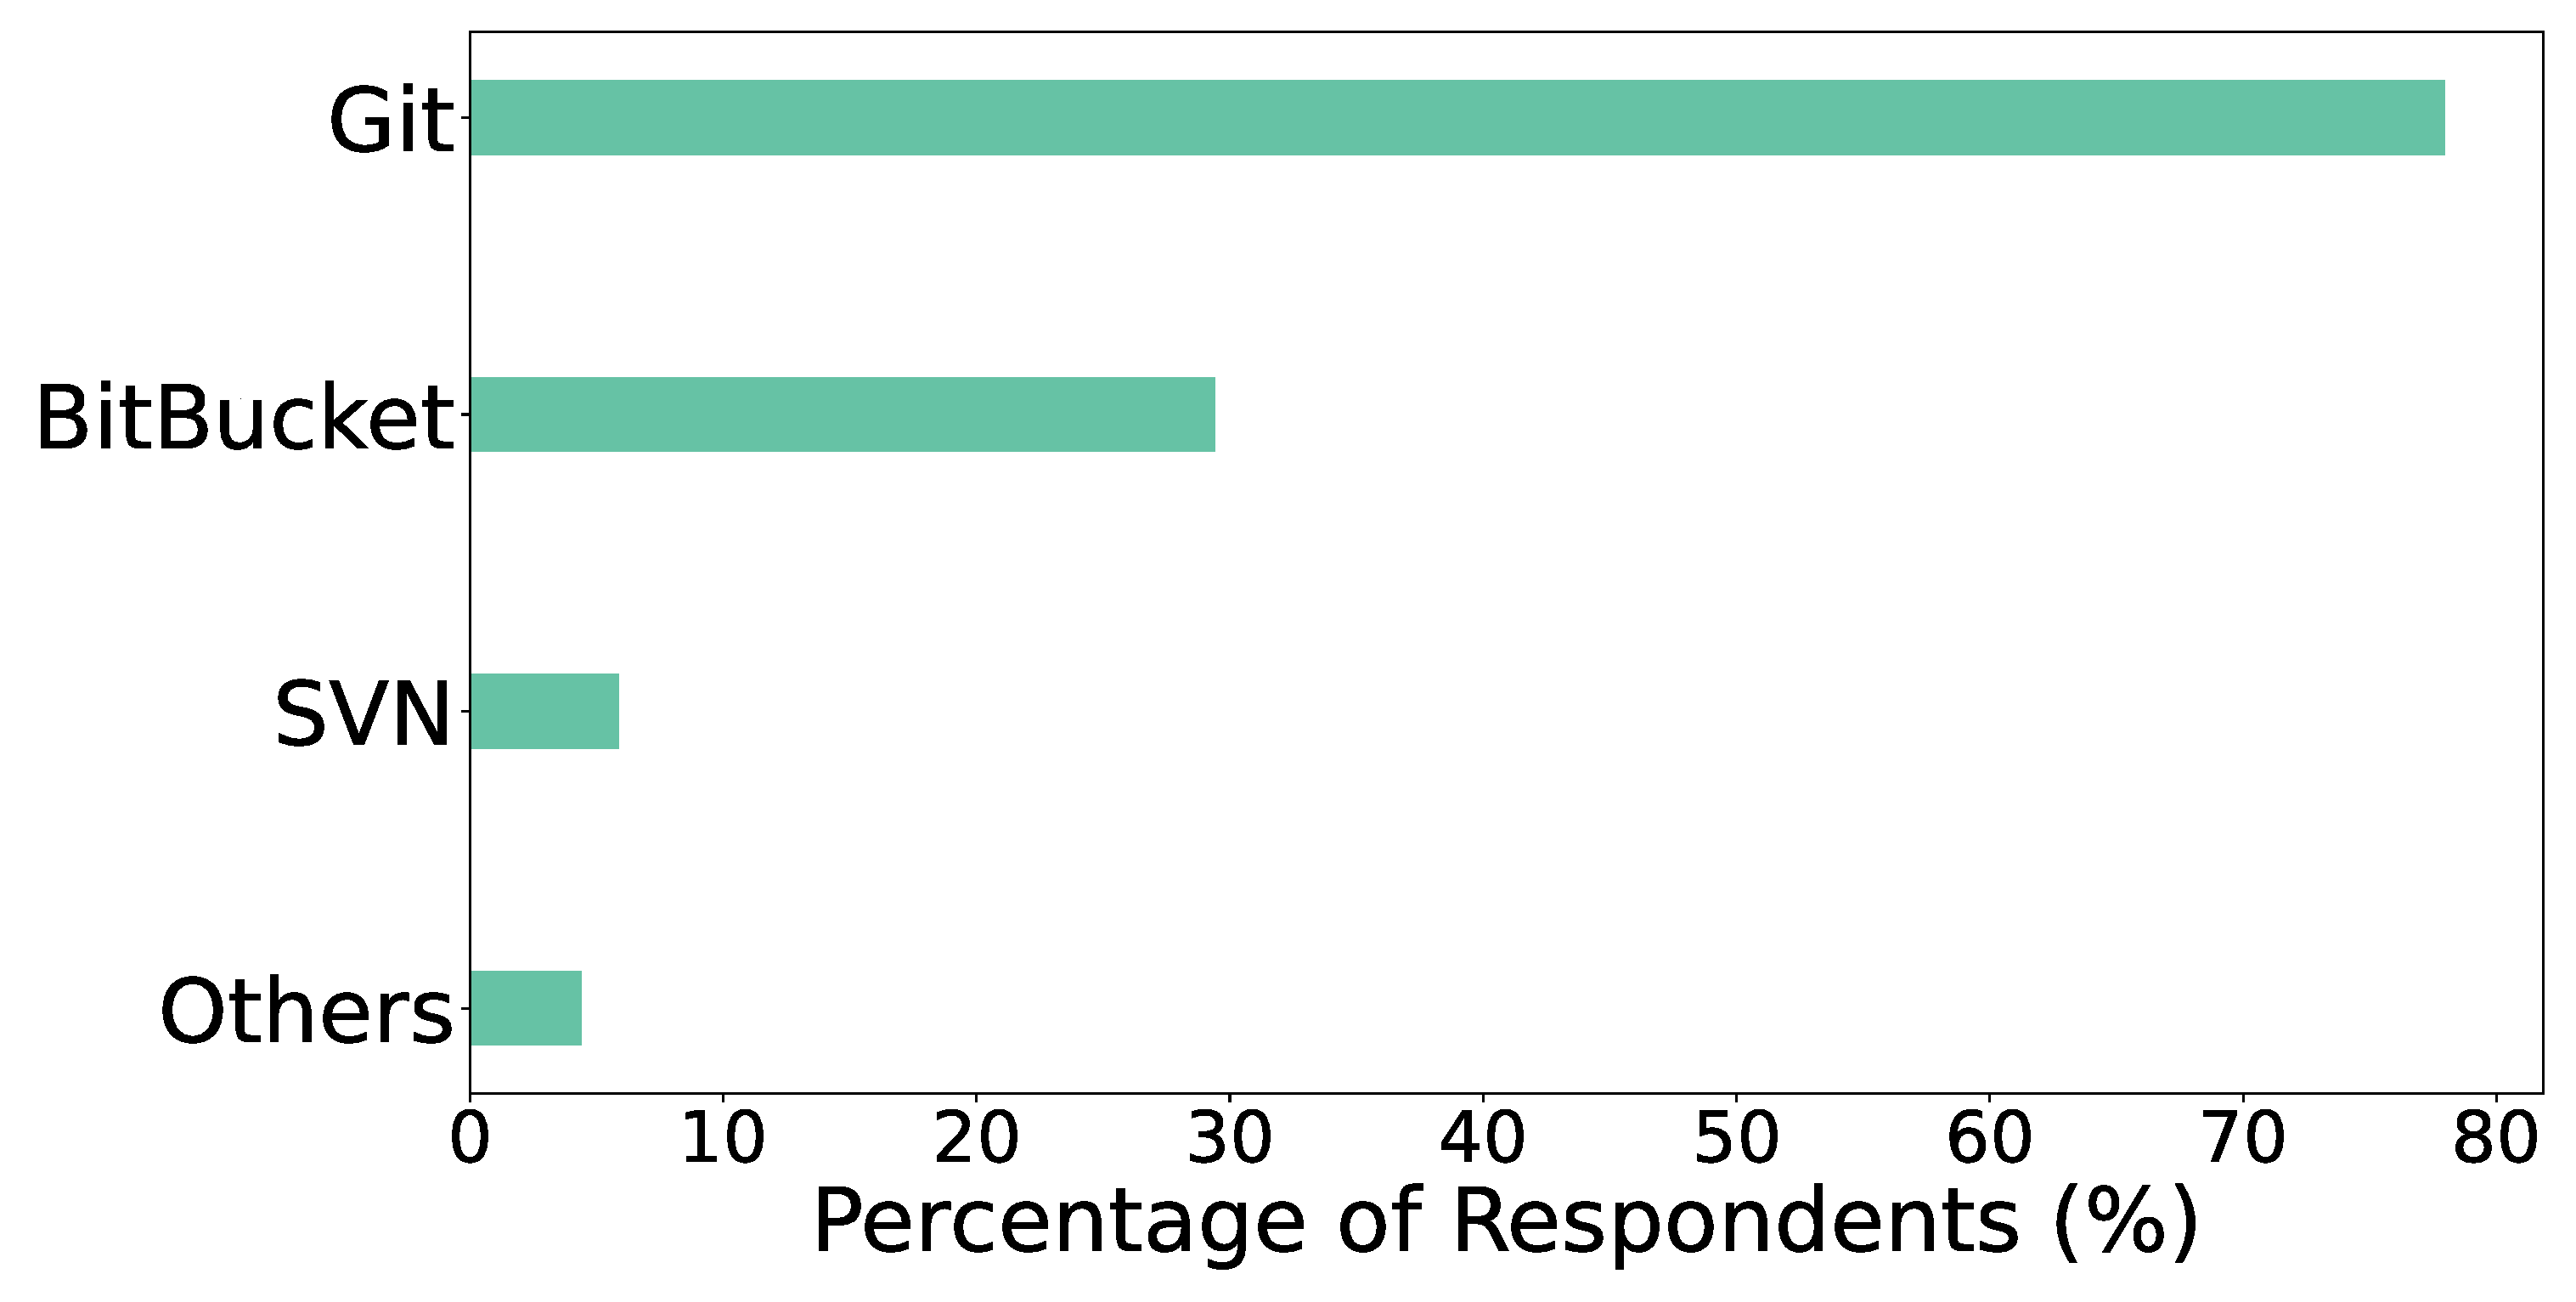
\includegraphics[scale=0.16]{Figures/Respondents_version_control}
  \caption{Version Control}
  \label{fig:versionControl}
\end{figure}
